\documentclass{beamer}
 
\usepackage[utf8]{inputenc}


\usetheme{Madrid}
\usecolortheme{default}
\usepackage{caption}
\usepackage{subcaption}
\usepackage{hhline}
\usepackage{graphicx}
\usepackage{physics}
\usepackage{amsmath}
\usepackage{amsfonts}
\usepackage{esint}
\usepackage{bbold}
\usepackage{mathtools}
\usepackage{dsfont}
\usepackage{amsthm}
\usepackage{bbm}
\usepackage{amssymb}
\theoremstyle{definition}
\newtheorem{defn}{Definition}[section]
\newtheorem{prop}{Properties}[section]
\newtheorem{rmk}{Remark}[section]
\newtheorem{exmp}{Example}[section]
\newtheorem{prob}{Problem}[section]
\newtheorem{proposition}{Proposition}
\newtheorem{thm}{Theorem}[section]
\newtheorem*{prob*}{Problem}
\newtheorem*{sln*}{Solution}
\usepackage{empheq}
\usepackage{tensor}

\newcommand{\lag}{\mathcal{L}}
\newcommand{\pOne}{\text{5p}_\text{1/2}}
\newcommand{\pThree}{\text{5p}_\text{3/2}}
\newcommand{\potassium}{^\text{39}\text{K}}
\newcommand{\R}{\mathbb{R}}
\newcommand{\lp}{\left(}
\newcommand{\rp}{\right)}
\newcommand{\lb}{\left[}
\newcommand{\rb}{\right]}
\newcommand{\lc}{\left\{}
\newcommand{\rc}{\right\}}
\newcommand{\p}{\partial}
\newcommand{\f}[2]{\frac{#1}{#2}}
\newcommand{\Vol}{\operatorname{Vol}}
\newcommand{\iprod}{\mathbin{\lrcorner}}
\newcommand{\al}{\alpha}
\newcommand{\be}{\beta}
\newcommand{\FT}{\mathcal{F}}
\newcommand{\LT}{\mathcal{L}}
\usepackage{hyperref}
\usepackage{tensor}
\usepackage{xcolor}
\hypersetup{
	colorlinks,
	linkcolor={black!50!black},
	citecolor={blue!50!black},
	urlcolor={blue!80!black}
}

% 3j symbol
\newcommand{\tj}[6]{ \begin{pmatrix}
		#1 & #2 & #3 \\
		#4 & #5 & #6 
\end{pmatrix}}
% 6j symbol
\newcommand{\Gj}[6]{ \begin{Bmatrix}
		#1 & #2 & #3 \\
		#4 & #5 & #6 
\end{Bmatrix}}

\setbeamerfont{title}{size=\large}

 
 
%Information to be included in the title page:
\title[\textcolor{white}{{Observation of vacuum-induced collective quantum beats}}]
{
	Observation of vacuum-induced collective quantum beats
}



\author[Bui] % (optional)
{Huan Q. Bui
	}

\institute[MIT] % (optional)
{
}
\date{ZGS, Jan 28, 2022}
 
%\logo{
\includegraphics[height=0.3cm]{colby.png}}
 
\begin{document}
 
\frame{\titlepage}



%%%%%%%%%%%%%%%%%%%%%%%%%%%%%%%%%%%%%%%%%%%%%%%%%%%%%%%%%%%%%%%%%%%%%%%%%

 
%\begin{frame}
%\frametitle{Layout}
%\tableofcontents
%\end{frame}

%%%%%%%%%%%%%%%%%%%%%%%%%%%%%%%%%%%%%%%%%%%%%%%%%%%%%%%%%%%%%%%%%%%%%%%%%




\begin{frame}
\textcolor{purple}{{Phys. Rev. Lett. \textbf{127}, 073604 – Published 13 August 2021}}
	\begin{figure}[!htb]
		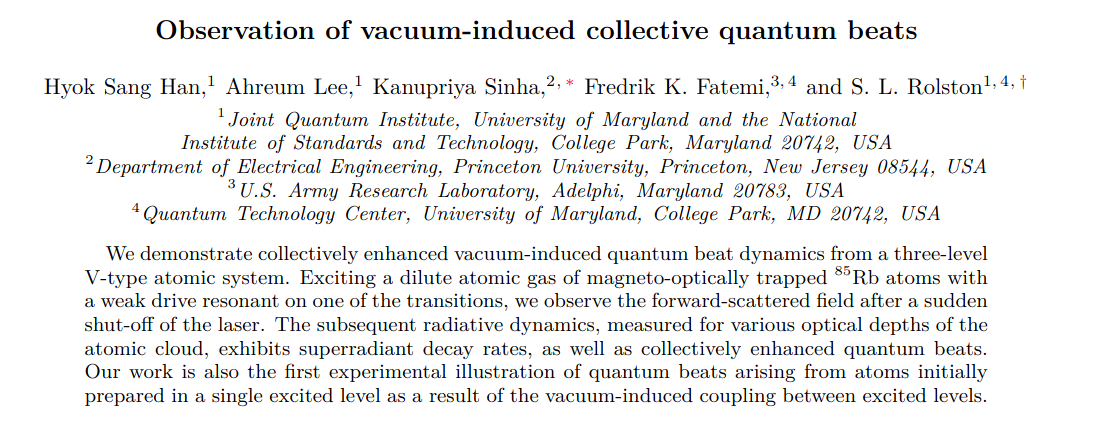
\includegraphics[width=1\textwidth]{abstract.png}
	\end{figure}
\end{frame}




\begin{frame}
\frametitle{Quantum beats}
\begin{itemize}
	\item Oscillatory behavior in the intensity of radiation emitted by atomic/molecular systems in a superposition of (excited) states
	
	\item Ex: quantum beats in the decay $\ket{5P_{3/2}}\to \ket{4S_{1/2}}$ in $^{39}$K
\end{itemize}




\begin{figure}[!htb]
	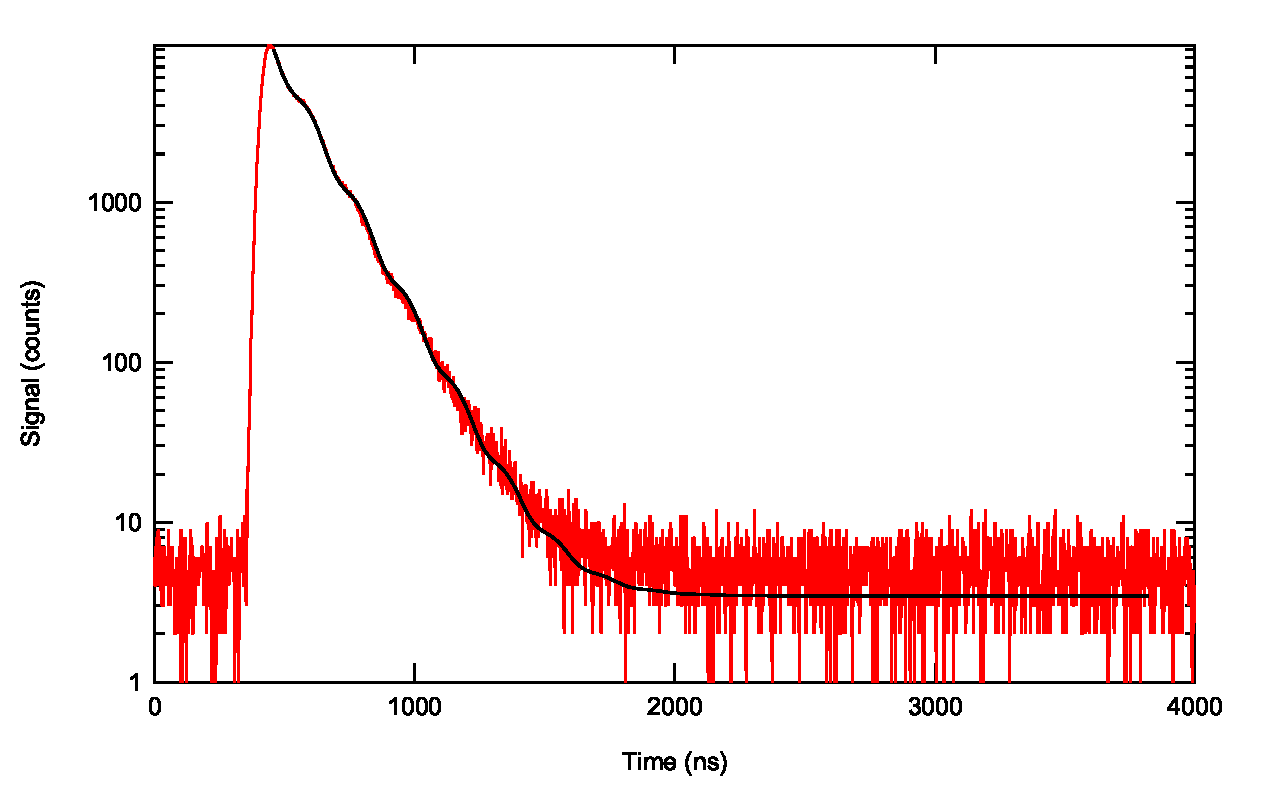
\includegraphics[width=0.6\textwidth]{big_beats_2.eps}
\end{figure}



\end{frame}




\begin{frame}



Simplest case is the three-level system. Two types: $V$ and $\Lambda$.

\begin{figure}[!htb]
	\begin{subfigure}{0.45\textwidth}
		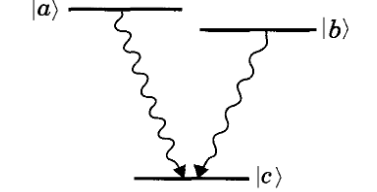
\includegraphics[width=\textwidth]{V.png}
	\end{subfigure}
	\begin{subfigure}{0.45\textwidth}
		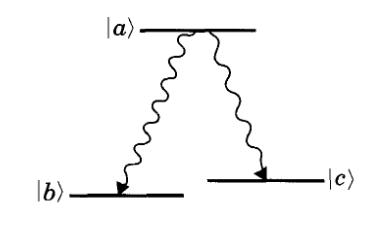
\includegraphics[width=\textwidth]{A.png}
	\end{subfigure}
\end{figure}


\begin{align*}
\ket{\psi_V(t)} &=  \sum_{i=a,b,c} \al_i \ket{i,0} + \al_1\ket{c,1_{\nu_1}} + \al_2 \ket{c,1_{\nu_2}}\\
\ket{\psi_\Lambda(t)} &=  \sum_{i=a,b,c} \al_i' \ket{i,0} + \al_1'\ket{b,1_{\nu_1}} + \al_2' \ket{c,1_{\nu_2}}
\end{align*}

\end{frame}


\begin{frame}
With
\begin{align*}
E^{(-)}_j(t) \sim a_j^\dagger e^{i\nu_j t} \quad \text{and} \quad E^{(+)}_j(t) \sim a_j e^{-i\nu_j t} 
\end{align*}
Beat note term:
\begin{equation*}
\bra{\psi_V(t)} E_1^{(-)}(t) E_2^{(+)}(t)  \ket{\psi_V(t)} \sim \bra{1_{\nu_1} 0_{\nu_2}} a_1^\dagger a_2 \ket{0_{\nu_1} 1_{\nu_2}} e^{i(\nu_1 - \nu_2)t} \underbrace{\braket{c}}_{1}
\end{equation*}

\begin{equation*}
\bra{\psi_\Lambda(t)} E_1^{(-)}(t) E_2^{(+)}(t)  \ket{\psi_\Lambda(t)} \sim \bra{1_{\nu_1} 0_{\nu_2}} a_1^\dagger a_2 \ket{0_{\nu_1} 1_{\nu_2}} e^{i(\nu_1 - \nu_2)t} \underbrace{\bra{c}\ket{b}}_{0}
\end{equation*}



\begin{itemize}
	\item Quantum beats exist in $V$-type systems in general, but not in $\Lambda$-type.
	
	
	\item Side note: This is not explained by semi-classical theory.
\end{itemize}

$\,$\\


\textcolor{purple}{\textbf{Textbooks: Quantum beats require a coherent superposition initially}}


\end{frame}



\begin{frame}
	\frametitle{"Observation of..." by Han et al.}
	
	Experimentally demonstrates 2 new aspects:
	\begin{itemize}
		\item \textbf{\textcolor{blue}{Vacuum-induced quantum beats:}} observed quantum beats without an initial superposition of excited levels
		
		
		\item \textbf{\textcolor{blue}{Collective effect:}} enhanced beat amplitudes 
	\end{itemize}
	
	
	
	
	
	
\end{frame}



\begin{frame}
	\frametitle{Experiment}
	
	\begin{figure}[!htb]
		\begin{subfigure}{0.55\textwidth}
			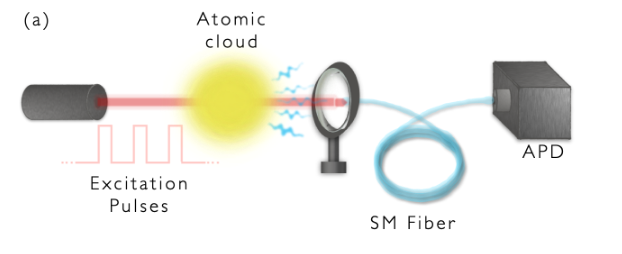
\includegraphics[width=\textwidth]{experiment.png}
		\end{subfigure}
		\begin{subfigure}{0.44\textwidth}
			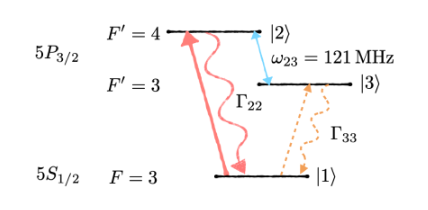
\includegraphics[width=\textwidth]{Rb85_levels.png}
		\end{subfigure}
	\end{figure}

\begin{itemize}
	\item $\sim 10^8$ $^{85}$Rb atoms in a MOT, $\rho \lambda^3 \ll 1$
	\item $V$-type system, well-separated. $\Gamma_{22} = 2\pi \cdot 6.1 $ MHz, $\Gamma_{33} = 5/9 \Gamma_{22}$
	\item $\Gamma_{23} \approx \sqrt{\Gamma_{22}\Gamma_{33}}$: 2nd order coupling between $\ket{2},\ket{3}$
	\item $v = 120 $ nm/\textmu s $\implies$ negligible to 780 nm over $1/\Gamma_{22}\approx 26$ ns
\end{itemize}
\end{frame}


\begin{frame}
	
	
	\begin{figure}[!htb]
		\begin{subfigure}{0.55\textwidth}
			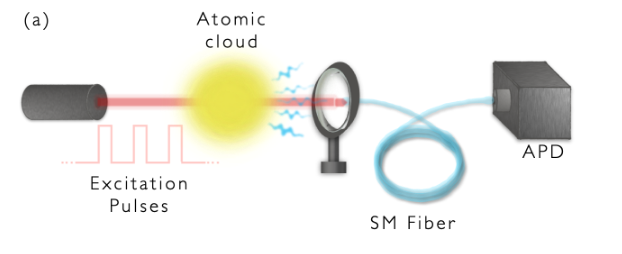
\includegraphics[width=\textwidth]{experiment.png}
		\end{subfigure}
		\begin{subfigure}{0.44\textwidth}
			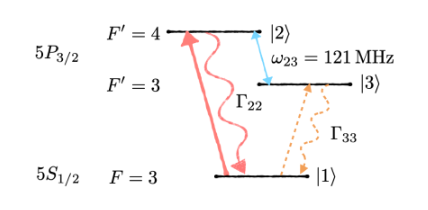
\includegraphics[width=\textwidth]{Rb85_levels.png}
		\end{subfigure}
	\end{figure}
	
\begin{itemize}
	\item Lin. pol. 780 nm light $(D_2)$ drives $\ket{1}\to \ket{2}$. 200 ns on, 800 ns off.  
	\item $> 30$ dB extinction ratio (2 EOMs in series), 3.5 ns fall time.
	\item $I_x \ll I_s = 3.9 \text{ mW/cm}^2 \implies$ single-excitation in $\ket{2}$
	\item Forward-photons collected by SM fiber into APD $\implies$ filters out incoherent fluorescence
	\item Histograms for $\sim$30 mins, new shot every 2 ms $\implies 2\times 10^8$ shots 
	
\end{itemize}
\end{frame}





\begin{frame}
	\frametitle{Data}
	
	\begin{figure}[!htb]
		\centering
		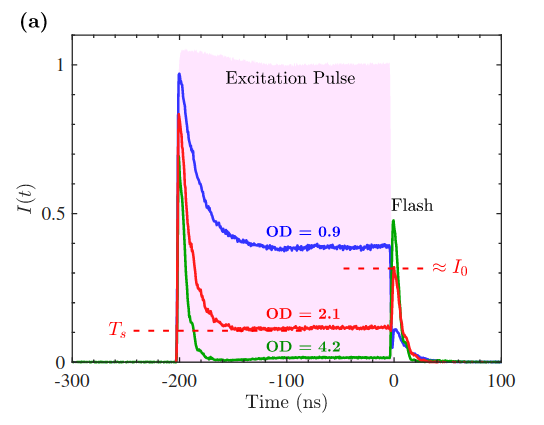
\includegraphics[width=0.6\textwidth]{data_full.png}
	\end{figure}
\end{frame}



\begin{frame}
	\frametitle{Data}
	
	\begin{figure}[!htb]
		\centering
		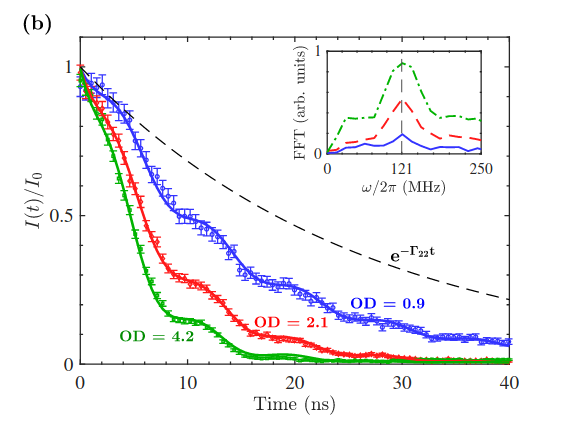
\includegraphics[width=0.6\textwidth]{data_zoom.png}
	\end{figure}

\begin{equation*}
\f{I(t)}{I_0} = e^{-\Gamma_{22}^{(N)}t} + I_b e^{-\Gamma_{\text{avg}}^{(N)}t} \sin(\omega_{23}t + \phi)
\end{equation*}
\end{frame}


\begin{frame}
	\frametitle{Data}
	
	\begin{figure}[!htb]
		\centering
		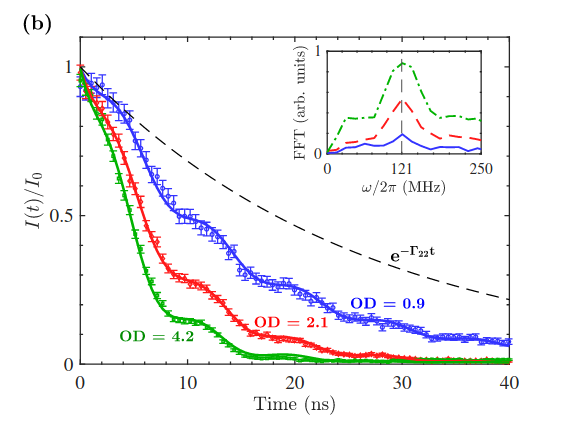
\includegraphics[width=0.6\textwidth]{data_zoom.png}
	\end{figure}
\end{frame}

\begin{frame}
	\frametitle{Data}
	
	\begin{figure}[!htb]
		\centering
		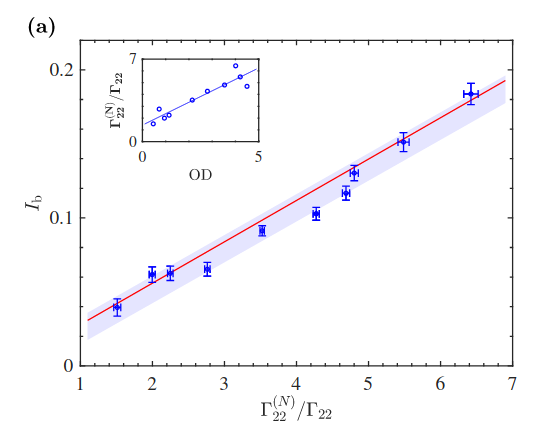
\includegraphics[width=0.6\textwidth]{data_Ib.png}
	\end{figure}
\end{frame}


\begin{frame}
	\frametitle{Model}
	
	\begin{equation*}
	\mathcal{H}
	\end{equation*}
\end{frame}


\begin{frame}
	\frametitle{Model vs. Data}
\end{frame}



\begin{frame}
	
	\frametitle{Conclusion}
	\textbf{Summary:}
	
	\begin{itemize}
		\item Demonstrated collective quantum beats in spontaneous emission process \textcolor{blue}{without} initial superposition of excited states
		
		\item Observed 
		\begin{itemize}
			\item enhanced decay rates ("superradiance")
			\item enhanced quantum beat amplitudes as a function of OD
		\end{itemize}
		Good agreement with theoretical model and previous studies.

	\end{itemize}


	$\,$\\
	\textbf{Applications:}
	\begin{itemize}
		\item Tool in precision spectroscopy: enhancing signals
		
		\item Combined with waveguide optics to study interactions between distant atomic ensembles (e.g. ONF experiment at JQI)
	\end{itemize}
\end{frame}



\begin{frame}
\frametitle{References}
\bibliographystyle{amsalpha}
\bibliography{references}{}
\end{frame}



\end{document}